\section{Deep model evaluation}
\label{sec:Deep model evaluation}
Due to the relatively short period for data collection in this study, from the beginning of 2021 June to the end of July, the total size of validly labelled videos collected was approximately 440MB.
By decoding these videos and videos randomly selected from the public data set Kinetics as the Unknown category into images, the total size of these images is approximately 2.3GB.

\begin{figure}[!ht]
    \centering
    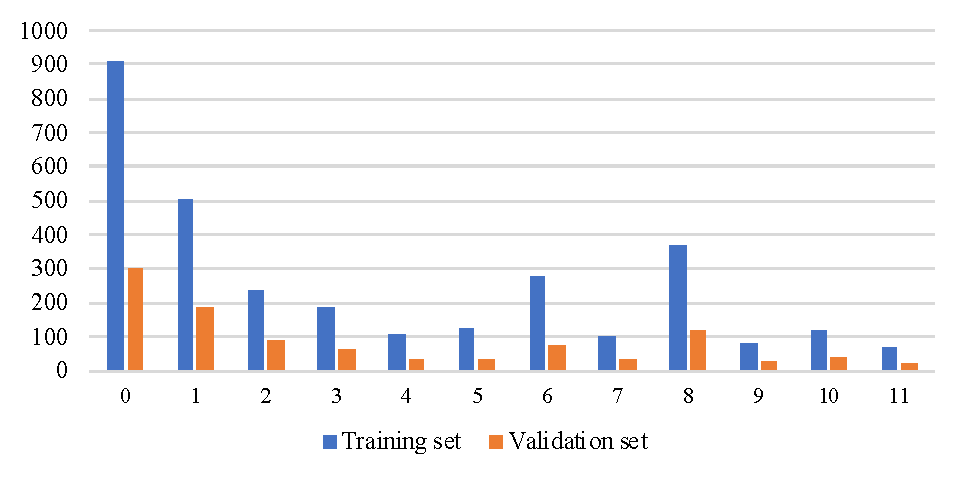
\includegraphics[width=\textwidth]{evaluation/imgs/5-data-dist-diag.pdf}
    \caption{Data per category distribution}
    \label{fig:5-data-dist-diag}
\end{figure}

Figure \ref{fig:5-data-dist-diag} shows the per-category data distribution after dividing the anonymised data into training and validation sets.
The horizontal axis of the histogram shows a total of 12 categories from 0 to 11.
Table \ref{tab:Model output} in the model design chapter introduced the definition of each category.
As for the vertical axis, it represents the number of labelled samples.
A labelled sample has one label and 16 frames from temporal sampling in a video clip.
To ensure that the validation data set has enough samples to illustrate the model performance, one-third of the total data set is divided into the validation data set, and the remaining two-thirds are used for training the deep model.

Overfitting is an unavoidable problem in deep learning, especially when using a complex model on small data sets.
It is a phenomenon that the model loses its generalisation application ability, which manifests as the model has extremely small loss and very high accuracy on the training set, however, a overfitted model will perform badly on the validation set. 
The main reasons for overfitting and the corresponding solutions are as follows:
\begin{enumerate}
    \item The size of the data set does not match the complexity of the model. \\ \textbf{Solution}: To use data augmentation or reduce the model complexity.
    \item There are errors in the data sets, e.g. data have wrong labels, unshuffled data resulting in distribution difference between the training set and the validation set. \\
    \textbf{Solution}: To visually inspect the data sets and ensure reliable data set labelling and distribution.
    \item Over-training, the model has been trained too much. \\
    \textbf{Solution}: To reduce the number of training epochs or use the early-stop mechanism to detect increasing loss in the validation set.
\end{enumerate}

In this study, the above three solutions are all applied in the training process to avoid overfitting.
In detail, the early-stop mechanism is implemented the model trainer, which monitors the loss value on the verification set after each training epoch.
Once the verification loss is found to increase, it will stop training.
The data loader uses common data augmentation methods in computer vision to perform the same transformation on the same batch of input data, such as scaling, randomly cropping, and flipping horizontally and vertically.
Besides, the data sets are carefully validated and visually checked using Jupyter notebook with \textit{matplotlib.animation} library.

Figure \ref{fig:5-lr-warmup} visually illustrates the result from the warm-up learning rate scheduler function introduced in the training hyperparameters design subsection \ref{subsec:Loss function and training hyperparameters}.
The figure covers the training iterations to 6000 as the training process is expected to be completed within 10 epochs.
Because this study uses a relatively small self-built data set and the deep model has a reduced complexity for mobile devices.
The figure shows that the learning rate increases linearly and reaches the peak at the 2000\textsuperscript{th} iteration, which is defined as a hyperparameter in the model trainer.
After the learning rate reaches its peak, it gradually decreases with a negative exponent, making the training process enter the final fine-tuning stage.

\begin{figure}[!htbp]
    \centering
    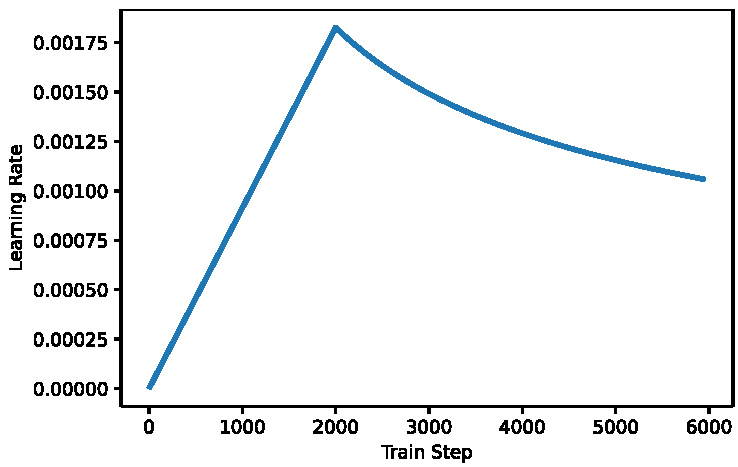
\includegraphics[width=.7\textwidth]{evaluation/imgs/5-lr-warmup.pdf}
    \caption{Learning rate warm-up}
    \label{fig:5-lr-warmup}
\end{figure}

Figure \ref{fig:5-train-step} and Figure \ref{fig:5-val-steps} display the model training and validating iterations.
At the beginning of the first epoch training, although the learning rate is low, the loss decreases steadily during this training epoch, indicating that the learning rate warm-up is effective to alleviate the overfitting.
If there was no learning rate warm-up mechanism, the training loss would drop dramatically at the beginning, and the loss might increase in the subsequent training process, indicating that the model was overfitted.
At the end of the first training epoch, the learning rate is about 0.00084, the loss drops to 1.92, and the accuracy on the training set achieves 0.4.
As for the validation after the first training epoch, both the loss and the accuracy is about 0.8 because no data augmentation applied to the validation data set, making this data set is easier to classify.

Starting from the second epoch, the training loss instantly drops to about 1, and the accuracy increases to 0.6 because all the training data has been completely input into the model once, thus, the model has already considerably understood the data form and distribution.
During the training process, the loss of the training data set is always dropping, but the loss in the validation data set starts to rise from epoch 4, which means that over-train the model leads to overfitting.
\vspace*{-.5em}
\begin{figure}[!ht]
    \centering
    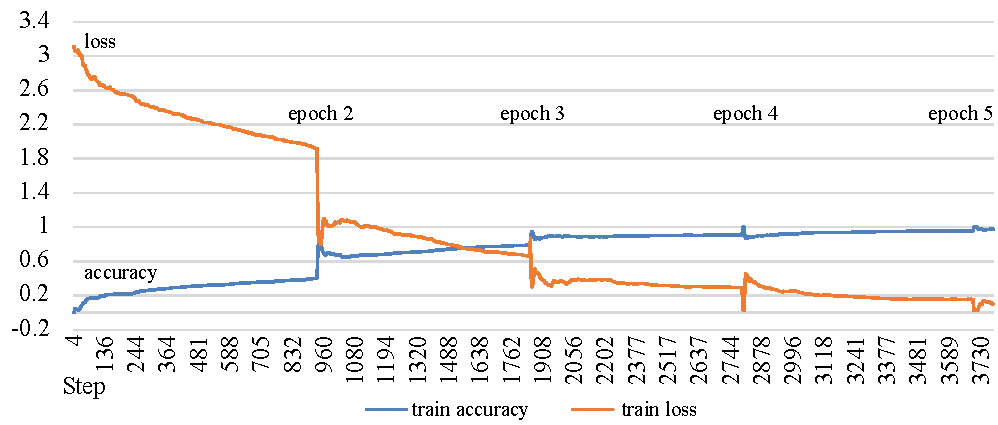
\includegraphics[width=.84\textwidth]{evaluation/imgs/5-train-step.pdf}
    \caption{Model training steps}
    \label{fig:5-train-step}
\end{figure}
\vspace*{-.5em}
\begin{figure}[!ht]
    \centering
    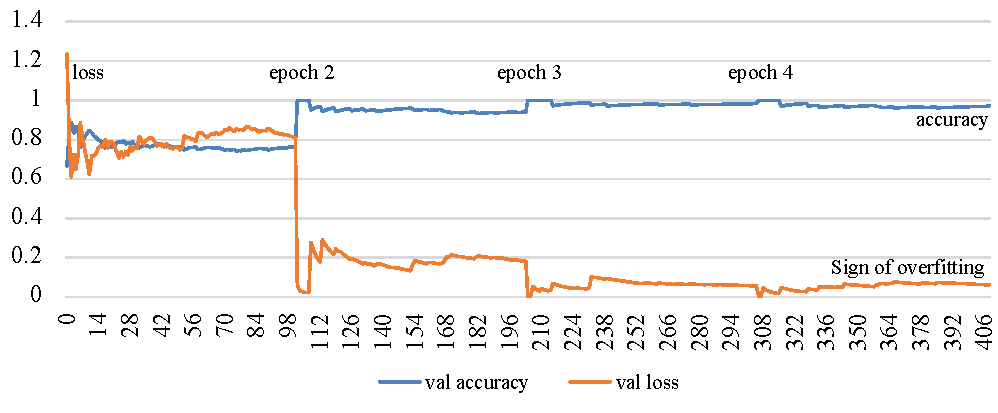
\includegraphics[width=.84\textwidth]{evaluation/imgs/5-val-steps.pdf}
    \caption{Model validation steps}
    \label{fig:5-val-steps}
\end{figure}

\clearpage
\begin{figure}[H]
    \centering
    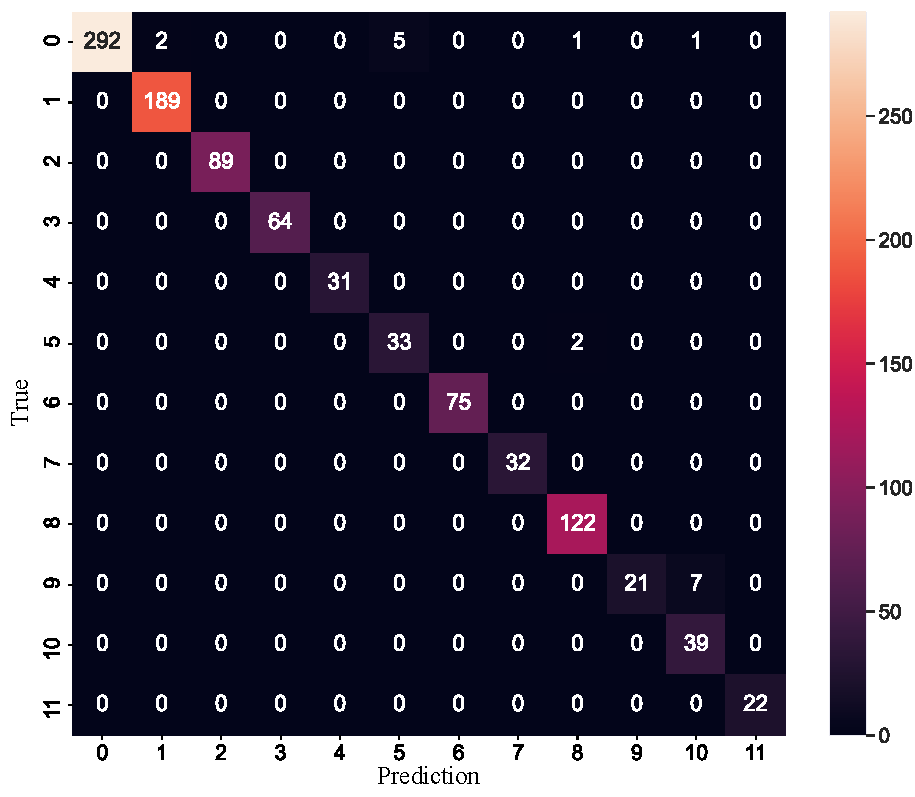
\includegraphics[width=.75\textwidth]{evaluation/imgs/5-confusion_matrix_val.pdf}
    \caption{Confusion matrix on validation data set}
    \label{fig:5-confusion_matrix_val}
\end{figure}
\begin{figure}[H]
    \centering
    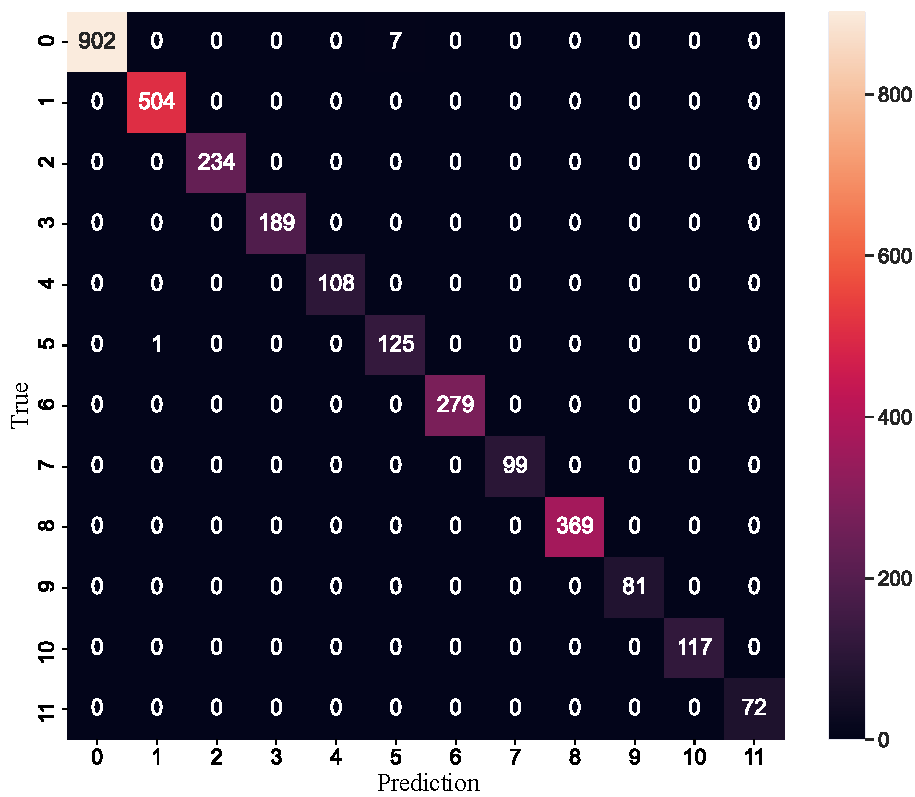
\includegraphics[width=.75\textwidth]{evaluation/imgs/5-confusion_matrix_train.pdf}
    \caption{Confusion matrix on training data set}
    \label{fig:5-confusion_matrix_train}
\end{figure}

Figure \ref{fig:5-confusion_matrix_val} and Figure \ref{fig:5-confusion_matrix_train} shows two confusion matrices on validation and training data set, respectively.
It is clear that most of samples are on the diagonal of the matrices, which means that they are classified correctly in both training and validation data set.
The validation result vitally reflects the model performance on samples that have not been used in the training process.

According to the formulae introduced in the evaluation metrics section \ref{sec:Evaluation metrics} above, Table \ref{tab:Classification report} shows a classification report of the validation data on Average Accuracy; Precision, Recall and F1-Score on macro average.
For those categories where precision and recall are 1.00, all samples in those categories are correctly classified.
This classification report highlights two data insights, first is that some samples from the Unknown category are classified to the other categories of exam activity, especially for the Leave category 5; second is that some samples labelled with 10 Drinking are classified to the 9 Scratching category.

\begin{table}[!htbp]
\centering
\begin{tabular}{|l|c|c|c|c|}
\hline
              & Precision & Recall & F1-Score & Support \\ \hline
0 Unknown     & 1.00      & \textbf{0.97}   & 0.98     & 301     \\ \hline
1 Look screen & 0.99      & 1.00   & 0.99     & 189     \\ \hline
2 Look down   & 1.00      & 1.00   & 1.00     & 89      \\ \hline
3 Look side   & 1.00      & 1.00   & 1.00     & 64      \\ \hline
4 Look back   & 1.00      & 1.00   & 1.00     & 31      \\ \hline
5 Leave       & \textbf{0.87}      & \textbf{0.94}   & 0.90     & 35      \\ \hline
6 Speaking    & 1.00      & 1.00   & 1.00     & 75      \\ \hline
7 Look up     & 1.00      & 1.00   & 1.00     & 32      \\ \hline
8 Use phone   & 0.98      & 1.00   & 0.99     & 122     \\ \hline
9 Scratching  & 1.00      & \textbf{0.75}   & 0.86     & 28      \\ \hline
10 Drinking   & \textbf{0.83}      & 1.00   & 0.91     & 39      \\ \hline
11 Typing     & 1.00      & 1.00   & 1.00     & 22      \\ \hline
Accuracy      & \multicolumn{3}{c|}{0.98}     & 1027    \\ \hline
macro avg     & 0.97      & 0.97   & 0.97     & 1027    \\ \hline
weighted avg  & 0.98      & 0.98   & 0.98     & 1027    \\ \hline
\end{tabular}
\caption{Classification report of validation data set}
\label{tab:Classification report}
\end{table}

As for the first data insight, the Unknown category has more false-negative results than the others, which means that some videos from the Unknown category were classified into the categories of exam activity.
Different proportions of the Unknown category to the exam activity categories will change the willingness of predicting the Unknown category.
In this study, the ratio of Unknown category size and the size of the total exam activity categories is $\frac{2940}{1210} = 0.42$.
In future works, more samples can be added into the Unknown category in the training data set to reduce false negatives in this category.

The second data insight is the misclassification between category 9 and category 10.
This problem is mainly due to insufficient training data and a certain similarity in these two categories.
For example, in both scratching and drinking activities, the participant needs to raise their hand first, do an action covering the face, and finally put their hand down.
If more training data is available in future work, the performance of these two categories can be easily improved.
